\chapter{التنفس الخلوي والتخمر}\label{ch:g12:respiration-fermentation}

عضلات عدّاء ماراثون تنفق، على مدى ثلاث ساعات ونصف، نحو نصف مول من \omterm{def:g12:respiration-fermentation:atp}{ATP}
في كل دقيقة --- أي ربع كيلوغرام من الجزيء، يصنع ويستعمل ويعاد صنعه
ألوف المرات من مخزون كان سيكفي خمس ثوان. وكل جزيء من جزيئات \omterm{def:g12:respiration-fermentation:atp}{ATP} تلك
يدفع ثمنه غلوكوز أو حمض دسم يفكك، ذرةً ذرةً، وجزيء أكسجين يستنشق في
البداية ويزفر ماء في النهاية. وقد أعطى \cref{ch:g10:cell-metabolism}
الحصيلة؛ وهذا الفصل يفتح \omterm{prop:g12:respiration-fermentation:mitochondrion}{المتقدرة} ويتابع الغلوكوز عبر المراحل الثلاث
التي تحول طاقته إلى \omterm{def:g12:respiration-fermentation:atp}{ATP} --- ويبين ماذا تفعل \omterm{def:g10:cells-common-unit:cell}{الخلية} حين ينفد الأكسجين.

\section{ATP، العملة}

\begin{definition}[ATP]\label{def:g12:respiration-fermentation:atp}
\emph{ATP}\index{ATP} (أدينوزين ثلاثي الفوسفات) \omterm{def:g10:universal-dna:nucleotide}{نوكليوتيد} يحمل ثلاث
مجموعات فوسفاتية على التوالي. ونزع الأخيرة منها يحرر نحو \qty{30}{kJ}
في المول في شروط \omterm{def:g10:cells-common-unit:cell}{الخلية}، وكل مسار في \omterm{def:g10:cells-common-unit:cell}{الخلية} يحتاج طاقة --- التقلص،
والنقل، والتركيب، وضوء اليراعة --- يقوده ذلك النزع. والناتج، وهو ADP،
يعاد شحنه ATP بتفاعلات هذا الفصل. وتحمل \omterm{def:g10:cells-common-unit:cell}{الخلية} ما يكفيها بضع ثوان من
ATP وتدوّره تدويرًا متصلًا؛ ويعيد إنسان مستريح تدوير ما يقارب كتلة جسمه
من ATP في يوم.
\end{definition}

\begin{proposition}[أين تكون الطاقة]\label{prop:g12:respiration-fermentation:oxidation}
الغلوكوز يخزن الطاقة في روابط الكربون--الهيدروجين عنده؛ وتحريرها يعني
نقل الهيدروجين، بإلكتروناته، إلى الأكسجين --- أي أكسدة الغلوكوز إلى
ثنائي أكسيد الكربون وإرجاع الأكسجين إلى ماء. ولو جرى ذلك في خطوة
واحدة، كما في اللهب، لغادرت الطاقة حرارةً. \omterm{def:g10:cells-common-unit:cell}{والخلية} تجريه في عشرات
الخطوات الصغيرة، يدير كل واحدة \omterm{def:g11:enzymes-and-phenotype:enzyme}{إنزيم}، وتلتقط جزءًا من الطاقة عند عدة
منها: فيحمَّل الهيدروجين أولًا على جزيئات حاملة --- هي \emph{NAD
المرجَع} --- ولا يسلَّم إلى الأكسجين إلا في النهاية.
\end{proposition}
\admitted

\section{ثلاث مراحل}

\begin{proposition}[تحلل السكر]\label{prop:g12:respiration-fermentation:glycolysis}
في \omterm{def:g10:cells-common-unit:cell}{السيتوبلازم}، بلا أكسجين، يشق غلوكوز (ست ذرات كربون) إلى جزيئين من
\emph{البيروفات} (ثلاث ذرات كربون لكل منهما) بعشر خطوات إنزيمية: وهو
\emph{تحلل السكر}\index{تحلل السكر}. والحصيلة: جزيئا \omterm{def:g12:respiration-fermentation:atp}{ATP} يستهلكان في
البدء، وأربعة تنتج، فالمكسب الصافي 2 \omterm{def:g12:respiration-fermentation:atp}{ATP}، وجزيئا NAD مرجَعين محمَّلين
بالهيدروجين. والبيروفات ما زال يحمل معظم طاقة الغلوكوز.
\end{proposition}
\admitted

\begin{proposition}[المتقدرة تتم الأكسدة]\label{prop:g12:respiration-fermentation:mitochondrion}
حين يتوافر الأكسجين، يدخل البيروفات \emph{المتقدرة}\index{متقدرة}،
وهي \omterm{def:g10:cells-common-unit:organelle}{عضية} يحدها غشاءان، الداخلي منهما مطوي إلى \emph{أعراف} تحيط
بالسائل الذي هو \emph{المادة الأساسية}.
\begin{itemize}
  \item في المادة الأساسية، يفكك كل بيروفات في دورة من التفاعلات، هي
        \emph{دورة كريبس}\index{دورة كريبس}: فتغادر ذراته الثلاث ثلاثة
        جزيئات $\mathrm{CO_2}$، ويحمَّل هيدروجينه على حاملين (NAD مرجَع
        وحامل ثانٍ)، ويصنع قليل من \omterm{def:g12:respiration-fermentation:atp}{ATP} مباشرة --- واحد لكل بيروفات.
  \item وفي الغشاء الداخلي، يسلّم الحاملان المحمَّلان إلكتروناتهما إلى
        سلسلة من \omterm{def:g10:chemistry-of-life:families}{البروتينات}، هي \emph{السلسلة التنفسية}، تمررها نزولًا
        إلى الأكسجين، فيتحد بالبروتونات ويكوّن ماء. والطاقة المتحررة
        على طول السلسلة تضخ بروتونات عبر الغشاء، وعودتها عبر \omterm{def:g11:enzymes-and-phenotype:enzyme}{إنزيم}
        دوار تقود تركيب \omterm{def:g12:respiration-fermentation:atp}{ATP} --- نحو 26 لكل غلوكوز.
\end{itemize}
والمجموع لغلوكوز واحد: نحو 30 \omterm{def:g12:respiration-fermentation:atp}{ATP} (اثنان من \omterm{prop:g12:respiration-fermentation:glycolysis}{تحلل السكر}، واثنان من
الدورة، ونحو 26 من السلسلة)، وستة جزيئات $\mathrm{CO_2}$ تتحرر، وستة
جزيئات $\mathrm{O_2}$ تستهلك، وما بقي من \qty{2870}{kJ} حرارةً.
\end{proposition}
\begin{proof}[شواهد]
\omterm{def:g10:cells-common-unit:organelle}{المتقدرات} المعزولة في حجرة محكمة فيها مسبار أكسجين لا تستهلك أكسجينًا
إذا أعطيت غلوكوزًا، لكنها تستهلكه بسرعة إذا أعطيت بيروفات --- \omterm{prop:g12:respiration-fermentation:mitochondrion}{فالمتقدرة}
لا تستطيع أن تبدأ من الغلوكوز؛ بل لا بد \omterm{def:g10:cells-common-unit:cell}{للسيتوبلازم} من ذلك. وإضافة سم
للسلسلة التنفسية (السيانيد) توقف الاستهلاك في الحال، أيًا كان \omterm{def:g11:enzymes-and-phenotype:enzyme}{الركيزة}
الحاضرة. وإضافة ADP تسرّع الاستهلاك ونفادها تبطئه: فاستعمال الأكسجين
مقترن بتركيب \omterm{def:g12:respiration-fermentation:atp}{ATP}. ومتقدرات عضلة طيران طائر الطنان أو فخذ عدّاء ماراثون
أعرافها أكثف بأضعاف من أعراف نسيج مستريح.
\end{proof}

\begin{omfigure}
\begin{tikzpicture}
  \node[anchor=south west, inner sep=0] (img) at (0,0)
    {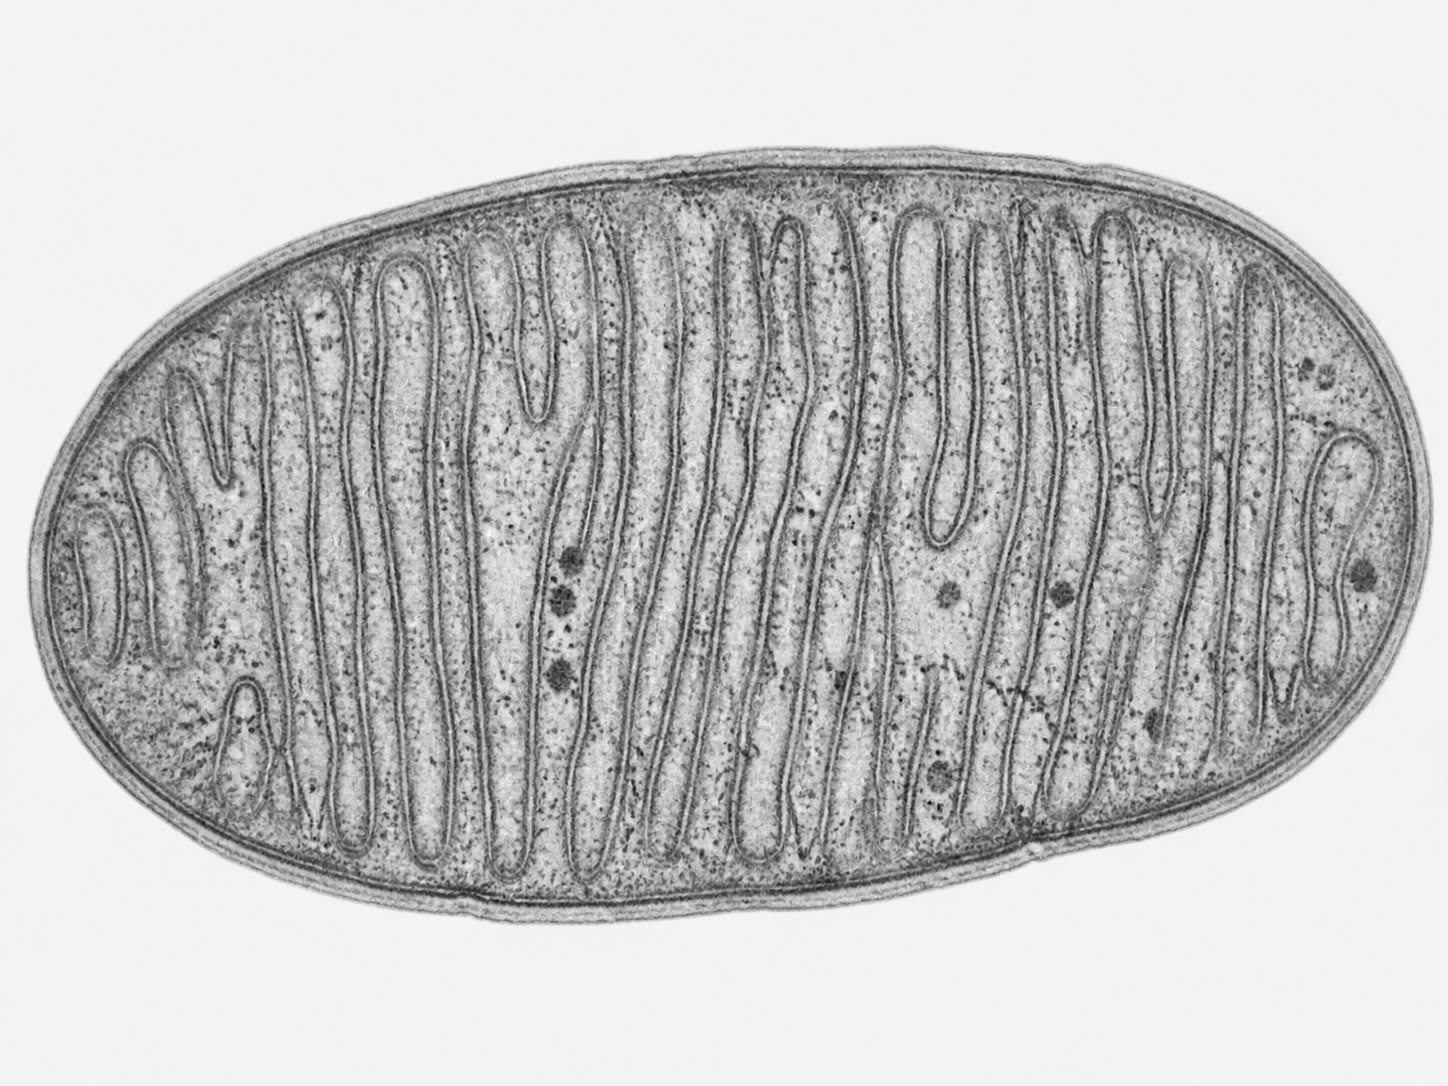
\includegraphics[width=0.5\linewidth]{images/book2/ai/g12-resp-mitochondrion-tem.jpg}};
  \begin{scope}[x={(img.south east)}, y={(img.north west)},
      every node/.style={font=\small}]
    \draw[omDef, thick] (0.08,0.55) -- (-0.04,0.80) node[left, align=right] {الغشاء\\ الخارجي};
    \draw[omDef, thick] (0.20,0.45) -- (-0.04,0.25) node[left, align=right] {الغشاء الداخلي،\\ مطويًا إلى أعراف};
    \draw[omDef, thick] (0.55,0.50) -- (0.55,-0.06) node[below] {المادة الأساسية (دورة كريبس)};
    \draw[omDef, thick] (0.80,0.60) -- (1.04,0.80) node[right, align=left] {الأعراف:\\ السلسلة التنفسية};
  \end{scope}
\end{tikzpicture}

{\small \omterm{def:g10:cells-common-unit:organelle}{متقدرة} في المجهر الإلكتروني. الغشاء الداخلي مطوي إلى أعراف،
تحمل السلسلة التنفسية \omterm{def:g11:enzymes-and-phenotype:enzyme}{والإنزيم} الذي يصنع \omterm{def:g12:respiration-fermentation:atp}{ATP}؛ والسائل بينها، وهو
المادة الأساسية، يدير \omterm{prop:g12:respiration-fermentation:mitochondrion}{دورة كريبس}.}
\end{omfigure}

\begin{omfigure}
\begin{tikzpicture}[font=\small, >=Stealth,
  b/.style={draw, rounded corners, align=center, minimum height=0.9cm}]
  % cytoplasm region
  \node[b, fill=omDef!8, minimum width=6.0cm, minimum height=6.2cm] (cyt) at (0,0) {};
  \node[anchor=north, font=\small\bfseries] at (cyt.north) {السيتوبلازم};
  \node[b, fill=omMeth!20, text width=2.4cm] (glu) at (0,2.0) {غلوكوز (6 C)};
  \node[b, fill=omProp!20, text width=2.4cm] (pyr) at (0,-0.2) {بيروفاتان\\ (3 C لكل منهما)};
  \draw[->, thick] (glu) -- node[right, align=left, font=\scriptsize] {تحلل السكر:\\ $+2$ ATP، و$+2$ NADH} (pyr);
  \node[b, fill=omThm!15, text width=2.6cm] (ferm) at (0,-2.4) {تخمر:\\ لاكتات، أو\\ إيثانول $+ \mathrm{CO_2}$};
  \draw[->, thick, omThm] (pyr) -- node[right, font=\scriptsize, align=left] {بلا $\mathrm{O_2}$:\\ NADH يتجدد} (ferm);
  % mitochondrion region
  \node[b, fill=omProp!8, minimum width=6.4cm, minimum height=6.2cm, rounded corners=14pt] (mit) at (7.3,0) {};
  \node[anchor=north, font=\small\bfseries] at (mit.north) {المتقدرة};
  \node[b, fill=omProp!20, text width=2.6cm] (krebs) at (7.3,1.4) {دورة كريبس\\ (المادة الأساسية):\\ $6\,\mathrm{CO_2}$ تخرج،\\ $+2$ ATP، والحاملان يحمَّلان};
  \node[b, fill=omThm!15, text width=2.8cm] (chain) at (7.3,-1.5) {السلسلة التنفسية\\ (الغشاء الداخلي):\\ الحاملان $+ \mathrm{O_2} \to \mathrm{H_2O}$،\\ $+26$ ATP};
  \draw[->, thick] (pyr.east) -- node[pos=0.72, above, font=\scriptsize] {مع $\mathrm{O_2}$} (krebs.west |- pyr.east);
  \draw[->, thick] (krebs) -- node[right, font=\scriptsize] {NAD المرجَع} (chain);
  \draw[->, thick] (10.9,-1.1) -- (chain.east |- 0,-1.1) node[pos=0, right] {$6\,\mathrm{O_2}$};
  \draw[->, thick] (chain.east |- 0,-1.9) -- (10.9,-1.9) node[right] {$6\,\mathrm{H_2O}$};
  \draw[->, thick] (krebs.east |- 0,1.8) -- (10.9,1.8) node[right] {$6\,\mathrm{CO_2}$};
\end{tikzpicture}

{\small مراحل التنفس الثلاث، ومختصر \omterm{def:g10:cell-metabolism:fermentation}{التخمر}. \omterm{prop:g12:respiration-fermentation:glycolysis}{تحلل السكر} في \omterm{def:g10:cells-common-unit:cell}{السيتوبلازم}
يعطي جزيئي \omterm{def:g12:respiration-fermentation:atp}{ATP} وبيروفاتين؛ وفي \omterm{prop:g12:respiration-fermentation:mitochondrion}{المتقدرة} تجرد \omterm{prop:g12:respiration-fermentation:mitochondrion}{دورة كريبس} البيروفاتين
إلى ثنائي أكسيد كربون وتحمّل الحاملين، وتفرغهما السلسلة التنفسية على
الأكسجين وهي تصنع معظم \omterm{def:g12:respiration-fermentation:atp}{ATP}. ومن غير أكسجين يحوَّل البيروفات إلى \omterm{def:g10:cell-metabolism:fermentation}{التخمر}،
وهو لا يعطي شيئًا زائدًا.}
\end{omfigure}

\begin{example}[قراءة أثر أكسجين]\label{ex:g12:respiration-fermentation:trace}
متقدرات معزولة في الحجرة: يبقى الأكسجين عند \qty{8}{mg/L}؛ ويضاف
الغلوكوز، فلا شيء؛ ويضاف البيروفات، فيهبط الأكسجين بمعدل
\qty{0.5}{mg/L} في الدقيقة؛ ويضاف ADP، فيشتد الهبوط إلى
\qty{1.5}{mg/L} في الدقيقة مدة، ثم يعود إلى \num{0.5}؛ ويضاف
السيانيد، فيتوقف الهبوط. أربع حقائق في أثر واحد: \omterm{prop:g12:respiration-fermentation:mitochondrion}{المتقدرة} تحتاج
البيروفات لا الغلوكوز؛ واستعمال الأكسجين مقترن بتركيب \omterm{def:g12:respiration-fermentation:atp}{ATP}؛ والاقتران
عبر السلسلة التي يسدها السيانيد؛ \omterm{prop:g12:respiration-fermentation:mitochondrion}{والمتقدرة} التي لا عمل لها تعمل على
الفارغ.
\end{example}

\begin{omfigure}
\begin{tikzpicture}
\begin{axis}[
  width=0.9\linewidth, height=5.6cm,
  axis x line=bottom, axis y line=left,
  xmin=0, xmax=16, ymin=0, ymax=10,
  xlabel={الزمن (min)}, ylabel={$\mathrm{O_2}$ المنحل (mg/L)},
  xlabel style={font=\small, at={(axis description cs:0.5,-0.12)}, anchor=north},
  ylabel style={font=\small},
  tick label style={font=\small}, xtick={0,2,4,6,8,10,12,14,16}, ytick={0,2,4,6,8},
  clip=false,
]
\addplot[thick, omThm] coordinates {(0,8) (2,8) (4,8) (6,7) (8,4) (10,3) (12,2) (14,2) (16,2)};
\draw[->, thick] (axis cs:2,9.6) -- (axis cs:2,8.4);
\node[font=\scriptsize, anchor=south] at (axis cs:2,9.7) {غلوكوز};
\draw[->, thick] (axis cs:4,9.6) -- (axis cs:4,8.4);
\node[font=\scriptsize, anchor=south] at (axis cs:4,9.7) {بيروفات};
\draw[->, thick] (axis cs:6,9.6) -- (axis cs:6,8.4);
\node[font=\scriptsize, anchor=south] at (axis cs:6,9.7) {ADP};
\draw[->, thick] (axis cs:12,9.6) -- (axis cs:12,8.4);
\node[font=\scriptsize, anchor=south] at (axis cs:12,9.7) {سيانيد};
\end{axis}
\end{tikzpicture}

{\small استهلاك الأكسجين عند متقدرات معزولة. الغلوكوز لا يفعل شيئًا؛
والبيروفات يبدأ الاستهلاك؛ وADP يسرّعه حتى ينفد؛ والسيانيد، وهو يسد
السلسلة التنفسية، يوقفه.}
\end{omfigure}

\section{بلا أكسجين: التخمر}

\begin{proposition}[التخمر يجدد الحامل]\label{prop:g12:respiration-fermentation:fermentation}
\omterm{prop:g12:respiration-fermentation:glycolysis}{تحلل السكر} يحمّل حاملي NAD لكل غلوكوز؛ ومع الأكسجين تفرغهما \omterm{prop:g12:respiration-fermentation:mitochondrion}{المتقدرة}.
ومن غير أكسجين كان الحاملان سيمتلئان في غضون ثوان ويتوقف \omterm{prop:g12:respiration-fermentation:glycolysis}{تحلل السكر}.
و\emph{التخمر}\index{تخمر} هو سبيل \omterm{def:g10:cells-common-unit:cell}{السيتوبلازم} إلى تفريغهما: فالبيروفات
نفسه يتلقى الهيدروجين ويصير إما \emph{لاكتات} (في \omterm{def:g10:cells-common-unit:cell}{خلايا} العضلة وجراثيم
الحليب) وإما \emph{إيثانولًا} (في الخميرة)، بعد أن يفقد
$\mathrm{CO_2}$. ولا يصنع \omterm{def:g12:respiration-fermentation:atp}{ATP} إضافي؛ فالمردود هو جزيئا \omterm{def:g12:respiration-fermentation:atp}{ATP} الآتيان من
\omterm{prop:g12:respiration-fermentation:glycolysis}{تحلل السكر}، أي نحو خمسة عشر ضعفًا أقل من مردود التنفس، والناتج ---
لاكتات أو إيثانول --- ما زال يحمل معظم طاقة الغلوكوز.
\end{proposition}
\admitted

\begin{omfigure}
\begin{tikzpicture}
\begin{axis}[
  ybar, bar width=22pt,
  width=0.7\linewidth, height=5.2cm,
  axis x line=bottom, axis y line=left,
  ymin=0, ymax=36, ylabel={ATP لكل غلوكوز},
  ylabel style={font=\small},
  symbolic x coords={تخمر, تحلل السكر + كريبس, تنفس كامل},
  xtick=data, tick label style={font=\small},
  enlarge x limits=0.3, ytick={0,10,20,30},
  nodes near coords, nodes near coords style={font=\small},
]
\addplot[fill=omThm!45, draw=omThm] coordinates {(تخمر,2) (تحلل السكر + كريبس,4) (تنفس كامل,30)};
\end{axis}
\end{tikzpicture}

{\small مردود \omterm{def:g12:respiration-fermentation:atp}{ATP} لكل غلوكوز. \omterm{prop:g12:respiration-fermentation:glycolysis}{تحلل السكر} وحده، مع \omterm{def:g10:cell-metabolism:fermentation}{التخمر} ليجدد حامله،
يعطي 2؛ \omterm{prop:g12:respiration-fermentation:mitochondrion}{ودورة كريبس} تضيف 2 مباشرة؛ والسلسلة التنفسية، وهي تحتاج
الأكسجين، تضيف الستة والعشرين الباقية.}
\end{omfigure}

\begin{example}[اختيار العضلة]\label{ex:g12:respiration-fermentation:muscle}
ليف عضلة عدّاء السرعة يحتاج \omterm{def:g12:respiration-fermentation:atp}{ATP} أسرع مما تستطيع متقدراته وإمداده
بالأكسجين أن يصنعا؛ \omterm{prop:g12:respiration-fermentation:glycolysis}{وتحلل السكر} مع \omterm{def:g10:cell-metabolism:fermentation}{التخمر} اللبني يسلّم \omterm{def:g12:respiration-fermentation:atp}{ATP} أسرع بثلاثة
أضعاف، بكلفة غلوكوز أعلى بخمسة عشر ضعفًا، وتتراكم اللاكتات حتى يوقف
الألم الجهد. أما ألياف عدّاءة الماراثون فتعمل بالتنفس، ببطء وإلى غير
نهاية تقريبًا، تحرق الدسم كما تحرق الغلوكوز؛ ومتقدراتها أكبر وأكثر
عددًا، وشعيراتها الدموية أكثف، ولاكتاتها تبقى منخفضة. وأنماط الألياف في
\cref{ch:g10:muscles-and-joints} هما هاتان الاستراتيجيتان مبنيتين في
\omterm{def:g10:cells-common-unit:cell}{الخلايا}.
\end{example}

\begin{method}[موازنة ميزانية طاقة]\label{met:g12:respiration-fermentation:budget}
\begin{enumerate}
  \item حوّل الاستطاعة اللازمة إلى \omterm{def:g12:respiration-fermentation:atp}{ATP}: فعند نحو \qty{30}{kJ} لكل مول
        من \omterm{def:g12:respiration-fermentation:atp}{ATP} قابلة للاستعمال، تكون \qty{1}{kW} من الاستطاعة
        الاستقلابية \qty{2}{mol} من \omterm{def:g12:respiration-fermentation:atp}{ATP} في الدقيقة.
  \item وحوّل \omterm{def:g12:respiration-fermentation:atp}{ATP} إلى وقود: 30 \omterm{def:g12:respiration-fermentation:atp}{ATP} لكل غلوكوز في التنفس، و2 في \omterm{def:g10:cell-metabolism:fermentation}{التخمر}.
  \item وحوّل الوقود إلى أكسجين: 6 $\mathrm{O_2}$ لكل غلوكوز يتنفس،
        و\qty{24}{L} لكل مول من الغاز.
  \item وقارن الأكسجين اللازم بما يسلّمه الدم
        (\cref{ch:g10:heart-lungs-effort}): والنقص يسده \omterm{def:g10:cell-metabolism:fermentation}{التخمر}،
        بلاكتاته.
\end{enumerate}
\end{method}

\begin{remark}[مرآة التركيب الضوئي]\label{rem:g12:respiration-fermentation:mirror}
\omterm{def:g10:cell-metabolism:autotrophy}{التركيب الضوئي} يحمّل إلكترونات من الماء على حاملين بالضوء ويستعملها في
إرجاع ثنائي أكسيد الكربون إلى سكر، محررًا الأكسجين؛ والتنفس يفرغ
إلكترونات من السكر على حاملين ويمررها إلى الأكسجين، فيصنع ماء ويحرر
ثنائي أكسيد الكربون، ويستعمل الطاقة في صنع \omterm{def:g12:respiration-fermentation:atp}{ATP}. وتدير الاثنين عضيتان
كانتا كلتاهما جرثومتين حرتين (\cref{ch:g12:diversification-of-life})،
\omterm{def:g12:photosynthesis:chloroplast}{والبلاستيدة الخضراء} تمد بما تستهلكه \omterm{prop:g12:respiration-fermentation:mitochondrion}{المتقدرة}؛ وهما معًا يحولان ضوء
الشمس إلى عملة كل \omterm{def:g10:cells-common-unit:cell}{خلية}، وأكسجين الجو هو رصيد حسابيهما.
\end{remark}

\section{تمارين}

\begin{exercise}[$\star$]\label{exo:g12:respiration-fermentation:1}
ما \omterm{def:g12:respiration-fermentation:atp}{ATP}، وماذا يحدث حين تستعمله \omterm{def:g10:cells-common-unit:cell}{خلية}؟
\end{exercise}

\begin{exercise}[$\star$]\label{exo:g12:respiration-fermentation:2}
سمّ مراحل التنفس الثلاث، وأين تقع كل واحدة، وماذا تعطي كل واحدة.
\end{exercise}

\begin{exercise}[$\star$]\label{exo:g12:respiration-fermentation:3}
صف \omterm{prop:g12:respiration-fermentation:mitochondrion}{المتقدرة} وقل أي مرحلة تجري في كل حجرة من حجراتها.
\end{exercise}

\begin{exercise}[$\star$]\label{exo:g12:respiration-fermentation:4}
ماذا يحقق \omterm{def:g10:cell-metabolism:fermentation}{التخمر} \omterm{def:g10:cells-common-unit:cell}{للخلية}، وماذا يعطي؟
\end{exercise}

\begin{exercise}[$\star$]\label{exo:g12:respiration-fermentation:5}
قارن مردود \omterm{def:g12:respiration-fermentation:atp}{ATP} في التنفس \omterm{def:g10:cell-metabolism:fermentation}{والتخمر}، والنواتج الباقية في نهاية كل منهما.
\end{exercise}

\begin{exercise}[$\star\star$]\label{exo:g12:respiration-fermentation:6}
من أثر الأكسجين، ماذا تبين كل إضافة من الإضافات الأربع؟
\end{exercise}

\begin{exercise}[$\star\star$]\label{exo:g12:respiration-fermentation:7}
لماذا لا تستطيع \omterm{def:g10:cells-common-unit:organelle}{المتقدرات} المعزولة أن تستعمل الغلوكوز، بينما تستطيع
\omterm{def:g10:cells-common-unit:cell}{خلية} كاملة؟
\end{exercise}

\begin{exercise}[$\star\star$]\label{exo:g12:respiration-fermentation:8}
فسّر لماذا كان \omterm{prop:g12:respiration-fermentation:glycolysis}{تحلل السكر} سيتوقف في غضون ثوان بلا أكسجين لو لم يوجد
\omterm{def:g10:cell-metabolism:fermentation}{التخمر}.
\end{exercise}

\begin{exercise}[$\star\star$]\label{exo:g12:respiration-fermentation:9}
\omterm{def:g10:cells-common-unit:cell}{خلية} تحتاج 60 \omterm{def:g12:respiration-fermentation:atp}{ATP} في الثانية. فكم جزيء غلوكوز في الثانية يكلفها ذلك
بالتنفس، وكم \omterm{def:g10:cell-metabolism:fermentation}{بالتخمر}؟
\end{exercise}

\begin{exercise}[$\star\star$]\label{exo:g12:respiration-fermentation:10}
السيانيد قاتل في غضون دقائق. فسّر لماذا، من السلسلة التنفسية، ولماذا
يخفق الدماغ والقلب أولًا.
\end{exercise}

\begin{exercise}[$\star\star$]\label{exo:g12:respiration-fermentation:11}
من أين يأتي ثنائي أكسيد الكربون الذي تزفره، مرحلةً مرحلةً؟ ومن أين
يأتي الماء الذي يصنعه التنفس؟
\end{exercise}

\begin{exercise}[$\star\star\star$]\label{exo:g12:respiration-fermentation:12}
عضلة تنتج لاكتات في سباق، ثم يعيد الكبد بعده تحويل اللاكتات إلى
غلوكوز مستعملًا \omterm{def:g12:respiration-fermentation:atp}{ATP} من التنفس. فسّر لماذا ينتهي الجسم كله إلى أن يكون
قد دفع أكثر من 30 \omterm{def:g12:respiration-fermentation:atp}{ATP} ثمنًا للغلوكوز الذي خمرته العضلة.
\end{exercise}

\begin{exercise}[$\star\star\star$]\label{exo:g12:respiration-fermentation:13}
الخميرة في الهواء تستعمل الغلوكوز ببطء ولا تصنع إيثانولًا؛ وإذا حبست
استعملته بسرعة وصنعت إيثانولًا. فسّر بالمردودات، وقل لماذا تنتفخ عجينة
الخبز سواء أكان للخميرة هواء أم لا.
\end{exercise}

\begin{exercise}[$\star\star\star$]\label{exo:g12:respiration-fermentation:14}
\omterm{def:g10:cells-common-unit:cell}{خلايا} الدهن البني عند مولود جديد تحوي متقدرات تعمل سلسلتها من غير أن
تصنع \omterm{def:g12:respiration-fermentation:atp}{ATP}: إذ يقصَّر تيار البروتونات. فماذا تنتج هذه \omterm{def:g10:cells-common-unit:cell}{الخلايا} بدل ذلك،
ولماذا كان ذلك نافعًا لمولود جديد؟
\end{exercise}

\begin{exercise}[$\star\star\star$]\label{exo:g12:respiration-fermentation:15}
قارن التنفس \omterm{def:g10:cell-metabolism:autotrophy}{والتركيب الضوئي} نقطةً نقطةً: مصدر الإلكترونات ومقصدها،
والغاز المستهلك والمتحرر، ودخل الطاقة وخرجها، \omterm{def:g10:cells-common-unit:organelle}{والعضية}. ثم قل في جملة
واحدة لماذا لا يستطيع أحدهما أن يوجد على الأرض من غير الآخر.
\end{exercise}

\section{مسألة: نصف مول من ATP في الدقيقة}

\begin{problem}[{مسألة نهاية الأسبوع --- طاقة عدّاءة تتابع من الواط
إلى الجزيء: ATP يعد، والغلوكوز والأكسجين يحسبان، وحصة المتقدرات تقاس،
والسرعة النهائية التي لا تستطيع السلسلة أن تدفع ثمنها}]
\label{pb:g12:respiration-fermentation:1}
تديم عدّاءة استطاعة استقلابية قدرها \qty{1000}{W}، يلتقط نحو ثلثها
\omterm{def:g12:respiration-fermentation:atp}{ATP}، ويغادر الباقي حرارةً. خذ \qty{30}{kJ} من الطاقة القابلة للاستعمال
لكل مول من \omterm{def:g12:respiration-fermentation:atp}{ATP}، و30 \omterm{def:g12:respiration-fermentation:atp}{ATP} لكل غلوكوز في التنفس و2 في \omterm{def:g10:cell-metabolism:fermentation}{التخمر}،
و\qty{2870}{kJ} لكل مول من الغلوكوز، و\qty{24}{L} لكل مول من الغاز،
والغلوكوز \qty{180}{g/mol}.

\medskip
\noindent\textbf{القسم الأول --- \omterm{def:g12:respiration-fermentation:atp}{ATP}.}
\begin{enumerate}
  \item كم مولًا من \omterm{def:g12:respiration-fermentation:atp}{ATP} تستعمل العدّاءة في الدقيقة؟ (ولا يعد إلا الثلث
        الملتقط \omterm{def:g12:respiration-fermentation:atp}{ATP}.)
  \item وأي كتلة ذلك من \omterm{def:g12:respiration-fermentation:atp}{ATP}، عند \qty{507}{g/mol}؟ قارنها بالغرامات
        القليلة التي تحملها العضلات في كل لحظة.
  \item وكم مرة في الدقيقة يعاد شحن كل جزيء \omterm{def:g12:respiration-fermentation:atp}{ATP}، إذا كان مخزون الجسم
        \qty{50}{g}؟
  \item ولو صنع ذلك \omterm{def:g12:respiration-fermentation:atp}{ATP} بالتنفس وحده، فكم مولًا من الغلوكوز كان
        يستهلك في الدقيقة؟
  \item وكم لترًا من الأكسجين في الدقيقة يقتضي ذلك؟ قارنه
        بقيمة $\dot V\!\mathrm{O_2}$max مقدارها \qty{4}{L/min}.
\end{enumerate}

\medskip
\noindent\textbf{القسم الثاني --- حصة \omterm{def:g10:cells-common-unit:organelle}{المتقدرات}.}
\begin{enumerate}[resume]
  \item من الثلاثين \omterm{def:g12:respiration-fermentation:atp}{ATP} لكل غلوكوز، كم واحدًا يصنع في \omterm{def:g10:cells-common-unit:cell}{السيتوبلازم} وكم
        في \omterm{prop:g12:respiration-fermentation:mitochondrion}{المتقدرة}؟ وأي كسر من \omterm{def:g12:respiration-fermentation:atp}{ATP} عند العدّاءة متقدري؟
  \item وكم مولًا من $\mathrm{CO_2}$ تزفر في الدقيقة، ومن أي مرحلة من
        مراحل التنفس تأتي؟
  \item وكم من \qty{2870}{kJ} في الغلوكوز ينتهي في \omterm{def:g12:respiration-fermentation:atp}{ATP}؟ وأين يذهب
        الباقي، وماذا تفعل العدّاءة بشأنه؟
  \item لمتقدرات عضلاتها مساحة غشاء داخلي كلية تبلغ نحو
        \qty{1000}{m^2}. فلماذا تحتاج السلسلة كل هذا السطح؟
  \item \omterm{def:g10:sport-and-health:training}{والتدريب} يضاعف متقدرات أليافها. فأي المقادير السابقة يغير ذلك،
        وأيها لا يغير؟
\end{enumerate}

\medskip
\noindent\textbf{القسم الثالث --- السرعة النهائية.}
في السرعة النهائية تحتاج عضلاتها \qty{800}{W} من الاستطاعة على صورة
\omterm{def:g12:respiration-fermentation:atp}{ATP} مدة 30 ثانية، بينما لا يستطيع التنفس، محدودًا بالأكسجين الذي يسلمه
الدم، أن يمد بأكثر من \qty{400}{W} على صورة \omterm{def:g12:respiration-fermentation:atp}{ATP}.
\begin{enumerate}[resume]
  \item كم مولًا من \omterm{def:g12:respiration-fermentation:atp}{ATP} تقتضي السرعة النهائية في المجموع؟
  \item وكم منه يستطيع التنفس أن يمد به في 30 ثانية، وكم لا بد أن يأتي
        من \omterm{def:g10:cell-metabolism:fermentation}{التخمر}؟
  \item وكم مولًا من الغلوكوز يستهلك الجزء المخمَّر، وكم مولًا من
        اللاكتات يترك؟
  \item قارن الغلوكوز المستعمل لكل \omterm{def:g12:respiration-fermentation:atp}{ATP} في الطريقين أثناء السرعة
        النهائية. ولماذا تقبل العضلة هذا الهدر؟
  \item وبعد السباق، تؤكسد اللاكتات أو تعاد غلوكوزًا. فسّر لماذا يبقى
        استهلاكها للأكسجين مرتفعًا دقائق عدة بعد أن تتوقف.
\end{enumerate}

\medskip
\noindent\textbf{القسم الرابع --- الوقود الآخر.}
يمد الدسم بنحو \qty{38}{kJ} في الغرام، ويحتاج، في الغرام، أكسجينًا
أكثر بنحو 20\% مما يحتاجه الغلوكوز للطاقة نفسها.
\begin{enumerate}[resume]
  \item لو جاء نصف \qty{1000}{W} عندها من الدسم، فأي كتلة دسم كانت
        ستحرق في الساعة؟
  \item ولماذا يعطي الدسم، مع أنه أغنى بالطاقة في الغرام، استطاعة أقل
        لكل لتر من الأكسجين؟
  \item الحموض الدسمة تدخل التنفس عند \omterm{prop:g12:respiration-fermentation:mitochondrion}{دورة كريبس}، متخطية \omterm{prop:g12:respiration-fermentation:glycolysis}{تحلل السكر}.
        فأي المراحل الثلاث لا يستطيع الدسم إذن أن يستعملها، وماذا
        يترتب على ذلك في السرعة النهائية؟
  \item ولماذا يظل الدماغ، وهو يعمل بالغلوكوز وحده، عاملًا أثناء
        السباق مع أن العضلات تأخذ معظم غلوكوز الدم؟
  \item اذكر النتيجة: مولات \omterm{def:g12:respiration-fermentation:atp}{ATP} التي تستعملها العدّاءة في الدقيقة،
        ولترات الأكسجين التي تدفع ثمنها، ومرحلة التنفس التي تصنع
        معظمها.
\end{enumerate}
\end{problem}
